\documentclass[12pt]{article}

\usepackage{pablo-devoir}
\usepackage[a5paper,margin=2cm]{geometry}

\pagestyle{empty}

\title{\large Fonctions affines Vecteurs}
\date{11/02/15}
\classe{2\up{des}14}
\dsnum{DS 5}

\begin{document}
\maketitle

\begin{exercice}[Fonctions affines --- 7 points]~
  \emph{On considère la fonction affine $f$ passant par les points $A\left( -2;1 \right)$ et $\left( 1;4 \right)$.}
  \begin{enumerate}
    \item 
      \begin{enumerate}
        \item \emph{Calculer l'équation de la fonction $f$.} Le coefficient directeur est $a=\frac{y_B-y_A}{x_B-x_A}=\frac{4-1}{1-\left( -2 \right)}=\frac{3}{3}=1$. Puisque le point $A$ fait partie de la fonction, on a $1=-2\times1+b$. La résolution de l'équation donne $b=3$. L'équation de la fonction est donc $f(x)=x+3$.
        \item \emph{La fonction est-elle croissante ou décroissante ?} Son coefficient directeur, 1, est positif, donc elle est croissante.
      \end{enumerate}
    \item 
      \begin{enumerate}
        \item \emph{Dresser le tableau de signes de la fonction $g:x\mapsto -3x+9$, définie sur $\mathbb{R}$.} La fonction est décroissante (car $-3<0$, donc elle est positive, puis négative. Elle change de signe en $-\frac{b}{a}=-\frac{9}{-3}=3$.
      \begin{center}
        \begin{tikzpicture}
          \tkzTabInit[lgt=2,espcl=2]
          {$x$ /1,
            $g(x)$ /1
          }
          {$-\infty$,$3$, $\infty$}%
          \tkzTabLine{, +, z ,-}
        \end{tikzpicture}
      \end{center}
        \item \emph{Sans calculer sa valeur, dire si $g(10)$ est positif ou négatif.} Puisque $10>3$, on lit sur le tableau de signes que $g(10)<0$.
      \end{enumerate}
  \end{enumerate}
\end{exercice}

\begin{exercice}[Parallélogramme --- 6 points]
  \emph{On considère un parallélogramme $ABCD$, et un point $E$ tel que $C$ soit le
  milieu de $\left[ BE \right]$, comme représentés sur la figure suivante.}

  \begin{center}
    \begin{tikzpicture}[very thick, scale=1]
      \coordinate (A) at (1, 2);
      \coordinate (B) at (0, 0);
      \coordinate (C) at (2, .3);
      \coordinate (D) at ($(A)+(C)-(B)$);
      \coordinate (E) at ($2*(C)-(B)$);

      \draw (A) node{$\bullet$} node[above left]{$A$};
      \draw (B) node{$\bullet$} node[below left]{$B$};
      \draw (C) node{$\bullet$} node[below]{$C$};
      \draw (D) node{$\bullet$} node[above right]{$D$};
      \draw (E) node{$\bullet$} node[below right]{$E$};

      \draw (A) -- (B) -- (C) -- (D) -- cycle;
    \end{tikzpicture}
  \end{center}
  \begin{enumerate}
    \item \emph{Justifier que $\vecteur{BC}=\vecteur{CE}$.} On sait que $C$ est le milieu de $\left[ BE \right]$, donc $\vecteur{BC}=\vecteur{CE}$.
    \item \emph{Quelle est la relation entre $\vecteur{AD}$ et $\vecteur{CE}$ ? Justifier.} Nous avons montré que $\vecteur{BC}=\vecteur{CE}$. De plus, puisque $ABCD$ est un parallélogramme, $\vecteur{BC}=\vecteur{AD}$. Donc $\vecteur{AD}=\vecteur{CE}$.
    \item \emph{En déduire la nature du quadrilatère $ADEC$.} C'est donc un parallélogramme.
  \end{enumerate}
\end{exercice}

\begin{exercice}[Placer des points --- 7 points]~
  \emph{On considère les points $A$, $B$, $C$ suivants.}
  \begin{center}
    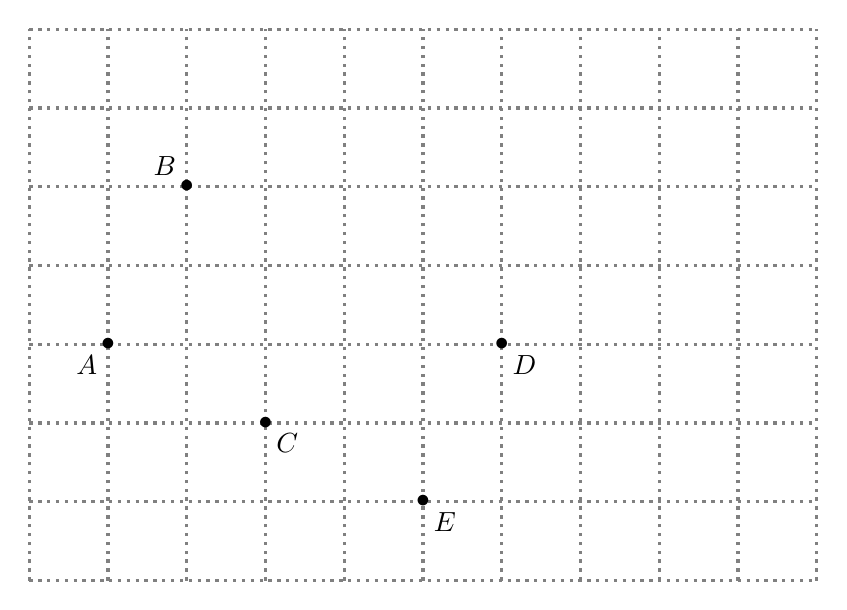
\begin{tikzpicture}[very thick]
      \draw[dotted, gray] (0,0) grid (10,7);
      \draw (1,3) node{$\bullet$} node[below left]{$A$};
      \draw (2,5) node{$\bullet$} node[above left]{$B$};
      \draw (3,2) node{$\bullet$} node[below right]{$C$};

      \draw (6,3) node{$\bullet$} node[below right]{$D$};
      \draw (5,1) node{$\bullet$} node[below right]{$E$};
    \end{tikzpicture}
  \end{center}
  \begin{enumerate}
    \item \emph{Placer le point $D$ tel que $\vecteur{BD}=2\vecteur{AC}$.} Voir la figure.
    \item \emph{On aimerait placer $E$ tel que $\vecteur{AE}=2\vecteur{CA}+2\vecteur{BD}$, mais placer ce point directement ferait sortir de la feuille. Nous allons faire autrement.}
      \begin{enumerate}
        \item \emph{Montrer que $\vecteur{CA}+\vecteur{BD}=\vecteur{AC}$.} On sait que $\vecteur{BD}=2\vecteur{AC}$.
          \begin{align*}
            \vecteur{BD} &= 2\vecteur{AC} \\
            \vecteur{BD} &= \vecteur{AC} + \vecteur{AC} \\
            \vecteur{BD} - \vecteur{AC} &= \vecteur{AC} + \vecteur{AC} - \vecteur{AC} \\
            \vecteur{BD} + \vecteur{CA} &= \vecteur{AC} \\
          \end{align*}
        \item \emph{En déduire que $\vecteur{AE}=2\vecteur{AC}$.}
          \begin{align*}
            \vecteur{AE} &= 2\vecteur{CA}+2\vecteur{BD} \\
            \vecteur{AE} &= 2\left(\vecteur{CA}+\vecteur{BD}\right) \\
            \vecteur{AE} &= 2\vecteur{AC} \\
          \end{align*}
        \item \emph{Placer enfin le point $E$.} Voir la figure.
      \end{enumerate}
  \end{enumerate}

\end{exercice}

\begin{exercice}[Bonus --- 1 points]
  \emph{
  Soient $A$ et $B$ deux points distincts. Lequel des deux vecteurs suivants a
  la plus grande norme : $\vecteur{AB}-\vecteur{BA}$, ou
  $\vecteur{AB}+\vecteur{BA}$ ? Justifier.
}

D'une part, on a : $\vecteur{AB}-\vecteur{BA}=\vecteur{AB}+\vecteur{AB}=2\vecteur{AB}$. Puisque $A$ et $B$ sont distincts, la norme de ce vecteur est donc deux fois la longueur $AB$. D'autre part, $\vecteur{AB}+\vecteur{BA}=\vecteur{AA}=\vecteur{0}$. Le vecteur nul a une norme nulle. Donc le premier vecteur a la plus grande norme.
\end{exercice}

\end{document}
